\section{Optimizer Algorithm}\label{sec:optimizer}

In this section, we discuss the algorithm to solve the optimization problem~(\ref{eq:glp:objective}).
Let $X \in \R^{n\times p}$, $y\in \R^n$ be the feature matrix and response vector, respectively.
Let $G$ be the number of groups and $p_i$ be the size of group $i$ for $1\leq i\leq G$.
Further let $X = \br{X_1 \, X_2 \, \ldots \, X_G}$ where $X_i \in \R^{n \times p_i}$ is the feature matrix
corresponding to group $i$ features only.

In general, if the loss function $f$ is of the form $f(\beta) \equiv f(y, X\beta)$,
the optimization problem~(\ref{eq:glp:objective}) can be reparametrized
in terms of $\tilde{\beta} \in \R^p$ where $\tilde{\beta}_i := Q_i^\top \beta_i$
where $Q_i \in \R^{p_i \times p_i}$ is the orthogonal matrix from the eigen-decomposition of 
$X_i^\top X_i = Q_i D_i Q_i^\top$ for each $i=1,\ldots, G$.
Concretely, it suffices to solve
\begin{align}
    \minimize_{\tilde{\beta} \in \R^p}
    f(y, \tilde{X} \tilde{\beta})
    + \lambda \sum\limits_{j=1}^G \norm{\tilde{\beta}_j}_2
    \label{eq:oa:new-objective}
\end{align}
where $\tilde{X} = \br{X_1 Q_1 \, X_2 Q_2 \, \ldots \, X_G Q_G}$.
Note that this was only possible because the group lasso penalty is invariant under
the transformation from $\beta \mapsto \tilde{\beta}$.
Then, given a solution $\tilde{\beta}^*$ to the new problem~(\ref{eq:oa:new-objective}),
we have the solution to the original problem $\beta^*$ given by
$\beta^*_i := Q_i \tilde{\beta}_i^*$.
Hence, without loss of generality, we assume that 
our feature matrix $X$ is of the form $\tilde{X}$.
In particular, we assume that $X_i^\top X_i = D_i$ is diagonal for all $1\leq i\leq G$.
We drop all tilde for notational simplicity.

Computationally, it may seem daunting to 
construct $\tilde{X}$ from $X$ before solving~(\ref{eq:oa:new-objective}).
However, the time taken for this pre-processing is relatively cheap compared to the full optimizing algorithm.
Given the data matrix $X$, consider a block $X_i \in \R^{n \times p_i}$.
we first perform the Singular Value Decomposition (SVD) such that
$X_i = U_iD_iV_i^T$ where $U_i \in \R^{n \times m_i}$, $D_i \in \R^{m_i \times p_i}$ and $V_i \in \R^{p_i \times p_i}$,
where $m_i = \min(n,p_i)$.
Note that $V_i$ is precisely the $Q_i$ from the preceding discussion.
Hence, $\tilde{X}_i \equiv U_i D_i$.
If $n \geq p_i$, then $\tilde{X}_i$ can be computed in $O(n p_i)$ time, noting that $D_i$ is diagonal.
Otherwise if $n < p_i$, then $D_i = [D_{i0} \; \textbf{0}_{n\times (p-n)}]$ where $D_{i0} \in \R^{n \times n}$ is the diagonal matrix.
Then, $\tilde{X}_i = [U_i D_{i0} \; \textbf{0}_{n \times (p-n)}]$ so that the only product to be computed takes $O(n^2)$ time.
Hence, the total complexity of the procedure is
\begin{align*}
    O\pr{
        \sum\limits_{i=1}^G
        \pr{\underbrace{\min(n,p_i) n p_i}_{\svd} + \underbrace{\min(n, p_i) n}_{\tilde{X}_i}}
    }
    =
    O\pr{
        n
        \sum\limits_{i=1}^G
        \min(n,p_i) p_i
    }
\end{align*}
Moreover, since this algorithm is parallelizable across groups,
we can reduce the time by the number of parallel threads.
This pre-computation complexity is smaller than the proposed optimizer algorithm\todojames{compute?}
and is a one-time computation.
Thus, it is worth performing this pre-computation for the large speed-ups in the optimizing algorithm.

In comparison to other proposed fitting procedures,
we believe that the extra cost to compute $\tilde{X}_i$, $D_i$, and $\tilde{X}_i^\top \tilde{X}_j$
is comparable to the cost of the other procedures.
For example, \citet{yuan:2006,meier:2008} rely on the fact that
each group feature matrix $X_i$ is full-rank and therefore admits a QR decomposition with an invertible $R$.
Under this assumption, they solve~(\ref{eq:oa:new-objective}) with $\tilde{X} = \br{Q_1 \, Q_2 \, \ldots \, Q_G}$
and transform the solution back to the original scale by applying $R_i^{-1}$ to the $i$th group of coefficients.
Note that this also applies a one-time decomposition of the group feature matrices.
The benefit of this approach is that the algorithm is aided by a simple closed-form expression
as part of the blockwise coordinate descent algorithm.
However, there are two major downsides to this approach.
The first is that, while the aforementioned authors primarily focused on the application of group lasso 
on multi-level categorical data that easily satisfy the full-rank assumption,
this assumption may easily be violated in other applications.
For example,~\todojames{mention GWAS; small n, bigger group size}.
The second is that this method only gives an approximation to the original problem.
That is, given the solution to~(\ref{eq:oa:new-objective}), $\tilde{\beta}^*$,
the candidate $\beta^\star$ defined by $\beta^\star_i := R_i^{-1} \tilde{\beta^\star}_i$ 
for $i=1,\ldots, G$ is not necessarily a solution to~(\ref{eq:glp:objective})
with the original data.
Indeed, for this approximation to be exact, 
rather than solving~(\ref{eq:oa:new-objective}),
one should solve
\begin{align*}
    \minimize_{\beta \in \R^p}
    f(y, \tilde{X} \tilde{\beta})
    + \lambda \sum\limits_{j=1}^G \norm{R_i^{-1} \tilde{\beta}_j}_2
\end{align*}
which introduces a Tikhonov regularization.
Although this remains a convex optimization problem and can be solved,
it does not simplify any computation since it does not enjoy the same 
closed-form expressions as the approximation method does.

Similar to other approaches~\citep{yuan:2006,meier:2008,tseng:2001,sparsegl:2022},
we use blockwise coordinate descent for its excellent speed and simplicity.
However, we take a completely different approach to fitting each block coordinate update.
The essence of implementing a highly performant optimizer lies in 
solving each block update~(\ref{eq:bcd:block-update}) as fast as possible.
Aside from the orthonormalization method described above as in~\citet{yuan:2006,meier:2008},
many works in literature that describe group lasso fitting procedures
use the general descent method called Proximal Gradient Descent (PGD), 
or Iterative Soft-Thresholding Algorithm (ISTA) in this context,
to solve~(\ref{eq:bcd:block-update})~\citep{sparsegl:2022,beck:2009,klosa:2020,wright:2009,loris:2009,sls:2016,odonoghue:2015}.
A Nesterov acceleration can be applied on ISTA to get Fast-ISTA (FISTA)~\citep{beck:2009}.
Further,~\citet{odonoghue:2015} showed that mild improvements can be made with an adaptive restarting strategy.
\Cref{ssec:bcd} describes the blockwise coordinate descent algorithm.
\Cref{ssec:pgd} describes the PGD (ISTA) procedure and its variations.
\Cref{ssec:newton,ssec:newton-abs} describe our proposed method to solve~(\ref{eq:bcd:block-update}).

\subsection{Blockwise Coordinate Descent}\label{ssec:bcd}

The convex optimization problem~(\ref{eq:oa:new-objective}) has a separable regularization,
so blockwise coordinate descent gives us guaranteed convergence~\citep{tseng:2001}.
Hence, we iterate through each block $j=1,\ldots, G$,
keeping all other blocks fixed, and solve the following problem:
\begin{align}
    \minimize_{\beta_j \in \R^{p_j}}
    f(y, X\beta)
    + \lambda \norm{\beta_j}_2
    \label{eq:bcd:block-problem}
\end{align}
until convergence is reached.
The final solution vector $\beta$ then solves~(\ref{eq:oa:new-objective}).

For the remainder of the paper, we only discuss the Gaussian loss~(\ref{eq:glp:gaussian}).
For a general $f$, we may apply Iterative Reweighted Least Squares (IRLS) 
by iteratively reweighting the data 
and solving~(\ref{eq:oa:new-objective}) with the Gaussian loss.
\todojames{Cite IRLS. Yuan and Meier?}
The Gaussian loss yields the optimization problem:
\begin{align*}
    \minimize_{\beta \in \R^p}
    \frac{1}{2} \norm{y - X \beta}_2^2 
    + \lambda \sum\limits_{j=1}^G \norm{\beta_j}_2
\end{align*}
with the block update for group $j$ as:
\begin{align*}
    \minimize_{\beta_j \in \R^{p_j}}
    \frac{1}{2} \beta_j^\top D_j \beta_j
    - (X_j^\top y - \sum\limits_{i \neq j} X_j^\top X_i \beta_i)^\top \beta_j
    + \lambda \norm{\beta_j}_2
\end{align*}
For notational simplicity, define $v_j := X_j^\top \pr{y - \sum\limits_{i \neq j} X_i \beta_i}$.
Then, dropping the subscript $j$, each block update is of the form:
\begin{align}
    \minimize_{\beta \in \R^p}
    \frac{1}{2} \beta^\top D \beta
    - v^\top \beta
    + \lambda \norm{\beta}_2
    \label{eq:bcd:block-update}
\end{align}
where $D \in \R^{p \times p}$ is diagonal with non-negative entries,
$v \in \R^p$ is any vector of the form $\sqrt{D} u$,
which follows from the fact that $X_j$ has the SVD of the form $U\sqrt{D}$ for an orthogonal matrix $U$ 
based on the discussion in~\Cref{sec:optimizer},
and $\lambda > 0$.

\subsection{Proximal Gradient Descent (PGD)}\label{ssec:pgd}

In this section, we describe the PGD method, or ISTA,
to solve the block update~(\ref{eq:bcd:block-update}).
The progression is similar to that of~\citet{sls:2016}.
Define
\begin{align*}
    f(\beta)
    &=
    \frac{1}{2} \beta^\top D \beta
    - v^\top \beta
\end{align*}
as the convex (Gaussian) loss function in~(\ref{eq:bcd:block-update}).
ISTA has guaranteed convergence so long as the step-size is chosen properly.
Any step-size $\nu$ can be chosen such that
$\nu \leq \frac{1}{L}$ where $L$ is the Lipschitz constant for $\nabla f$.
Since 
\begin{align*}
    \nabla f(\beta)
    &=
    D \beta - v
    \\\implies
    \norm{
        \nabla f(\beta)
        - \nabla f(\tilde{\beta})
    }_2
    &=
    \norm{D (\beta - \tilde{\beta})}_2
    \leq
    \opnorm{D} \norm{\beta-\tilde{\beta}}_2
\end{align*}
we have $L \equiv \opnorm{D} \equiv \lambda_{\max}(D)$ as the largest eigenvalue of $D$.
In particular, since $D$ is diagonal, $L \equiv \max\limits_{i} D_{ii}$.

The ISTA procedure is given in Algorithm~\ref{alg:pgd:ista}.
By applying a standard Nesterov acceleration~\citep{beck:2009}, 
we have the FISTA procedure given in Algorithm~\ref{alg:pgd:fista}.
Additionally, we may perform adaptive restarts
based on the proximal gradient updates~\citep{odonoghue:2015}
for even faster convergence as outlined in Algorithm~\ref{alg:pgd:fista-adares}.

\begin{algorithm}
    \caption{ISTA}\label{alg:pgd:ista}
    \KwData{$D$, $v$, $\lambda$, $\beta^{(0)}$}
    $\nu \gets \pr{\max\limits_{i} D_{ii}}^{-1}$\;
    \While{not converged}{
        $w \gets \beta^{(k-1)} + \nu \pr{v - D \beta^{(k-1)}}$\;
        $\beta^{(k)} \gets \pr{1-\frac{\nu\lambda}{\norm{w}_2}}_{+} w$\;
    }
\end{algorithm}

\begin{algorithm}
    \caption{FISTA}\label{alg:pgd:fista}
    \KwData{$D$, $v$, $\lambda$, $\beta^{(0)}$}
    $\nu \gets \pr{\max\limits_{i} D_{ii}}^{-1}$\;
    $\eta^{(1)} \gets \beta^{(0)}$\;
    $t_1 = 1$\;
    \While{not converged}{
        $w \gets \eta^{(k)} + \nu \pr{v - D \eta^{(k)}}$\; 
        $\beta^{(k)} \gets \pr{1-\frac{\nu\lambda}{\norm{w}_2}}_{+} w$\;
        $t_{k+1} \gets \frac{1 + \sqrt{1 + 4t_{k}^2}}{2}$\;
        $\eta^{(k+1)} \gets \beta^{(k)} + \frac{t_k-1}{t_{k+1}} (\beta^{(k)} - \beta^{(k-1)})$\;
    }
\end{algorithm}

\begin{algorithm}
    \caption{FISTA with Adaptive Restart}\label{alg:pgd:fista-adares}
    \KwData{$D$, $v$, $\lambda$, $\beta^{(0)}$}
    \While{not converged}{
        Carry out Algorithm~\ref{alg:pgd:fista} with 
        inputs $D$, $v$, $\lambda$, $\beta^{(0)}$ until
        \begin{align}
            \nabla f(\eta^{(k)})^\top (\beta^{(k)} - \beta^{(k-1)}) > 0
            \label{eq:fista-adares:cond}
        \end{align}
        \;
        \If{(\ref{eq:fista-adares:cond}) holds at step $k$} {
            Reset $\beta^{(0)} \gets \beta^{(k)}$\;
        }
    }
\end{algorithm}

Note that the computational cost of 
\Cref{alg:pgd:ista,alg:pgd:fista,alg:pgd:fista-adares}
are all $O(p k)$ where $k$ is the number of iterations until convergence.
Since we must output a vector in $\R^p$, 
any optimizer must necessarily have $O(p)$ operations.
Hence, the optimal optimizer of complexity $O(pk)$ must prioritize lowering 
the number of iterations until convergence.
While each algorithm is an improvement from the previous,
there is still much improvement left.
\Cref{ssec:newton} shows a novel approach to solving~(\ref{eq:bcd:block-update})
with a significant decrease in iterations while maintaining $O(p)$ operations per iteration.


\subsection{Newton's Method}\label{ssec:newton}

In this section, we propose a novel and simple method to solve~(\ref{eq:bcd:block-update}).
By solving the sub-gradient problem of~(\ref{eq:bcd:block-update}),
we see that the solution $\beta^\star$ must satisfy
\begin{align}
    \beta
    &=
    \begin{cases}
    \pr{D + \frac{\lambda}{\norm{\beta}_2} I}^{-1} v ,& \norm{v}_2 > \lambda \\
    0 ,& \norm{v}_2 \leq \lambda
    \end{cases}
    \label{eq:newton:block-solution}
\end{align}
Without loss of generality, we consider the first case when $\beta^\star \neq 0$.
Without knowing $\norm{\beta^\star}_2$, there is no closed-form solution for $\beta^\star$.
In an endeavor to find an expression for $\norm{\beta^\star}_2$,
we take the $\ell_2$ norm on both sides to get that $\norm{\beta^\star}_2$ must satisfy
\begin{align}
    \sum\limits_{i=1}^p
    \frac{v_i^2}{(D_{ii} \norm{\beta}_2 + \lambda)^2}
    =
    1
    \label{eq:newton:norm-solution}
\end{align}
Unfortunately, there is no closed-form solution for~(\ref{eq:newton:norm-solution}) either.
However, we will shortly show that there is an efficient algorithm 
to numerically solve~(\ref{eq:newton:norm-solution}).
In turn, once we find $\norm{\beta^\star}_2$, we may substitute it
into~(\ref{eq:newton:block-solution}) to get the full solution $\beta^\star$ in $O(p)$ time.
We note in passing that~(\ref{eq:newton:block-solution}) and~(\ref{eq:newton:norm-solution})
were previously discovered~\citep{sls:2016},
however, there is no mention of how to quickly solve for $\beta^\star$ or $\norm{\beta^\star}_2$.

We now discuss how to solve~(\ref{eq:newton:norm-solution}).
First, define $\varphi : [0, \infty) \to \R$ by
\begin{align*}
    \varphi(h)
    &:=
    \sum\limits_{i=1}^p
    \frac{v_i^2}{(D_{ii} h + \lambda)^2}
    - 1
\end{align*}
so that~(\ref{eq:newton:norm-solution}) is now a root-finding problem for $\varphi$.
Upon differentiating $\varphi$,
\begin{align*}
    \frac{d\varphi(h)}{dh}
    &=
    -2 \sum\limits_{i=1}^p
    \frac{v_i^2 D_{ii}}{(D_{ii} h + \lambda)^3}
    \leq
    0
\end{align*}
where the inequality is strict if not all $v_i^2 D_{ii} = 0$.
Note that if all $v_i^2 D_{ii} = 0$, then we must have that $\norm{v}_2 \leq \lambda$.
Otherwise,
\begin{align*}
    \varphi(h)
    &=
    \sum\limits_{i : D_{ii} = 0}
    \frac{v_i^2}{\lambda^2}
    - 1
    =
    \lambda^{-2} \sum\limits_{i=1}^p v_i^2 - 1
    > 0
\end{align*}
In particular, $\varphi$ is constant and strictly positive so it has no roots.
So, if $\norm{v}_2 > \lambda$, then there exists a vector $\beta$
where $\varphi(\norm{\beta}_2) = 0$, which is a contradiction.
Hence, without loss of generality, we may assume $\varphi'$ is strictly negative,
so that $\varphi$ is strictly decreasing.
Consequently, since $\varphi(0) > 0$ by hypothesis, there exists a (unique) root.
Further, it is easy to see that $\varphi$ is convex since it is a 
sum of convex functions.

Since $\varphi$ is convex, this suggests solving~(\ref{eq:newton:norm-solution})
via a one-dimensional Newton's Method.
Specifically, with $h^{(0)}$ as the initial starting point, for $k\geq 1$,
\begin{align}
    h^{(k)} = h^{(k-1)} - \frac{\varphi(h^{(k-1)})}{\varphi'(h^{(k-1)})}
    \label{eq:newton:newton-step}
\end{align}
We claim that Newton's Method is guaranteed to converge for any initial point $h^{(0)}$.
Indeed, for every $k\geq 1$, by convexity of $\varphi$,
\begin{align*}
    \varphi(h^{(k)})
    &\geq
    \varphi(h^{(k-1)})
    + \varphi'(h^{(k-1)}) (h^{(k)} - h^{(k-1)})
    =
    0
\end{align*}
Along with~(\ref{eq:newton:newton-step}),
this shows that $h^{(k)}$ is an increasing sequence for $k\geq 1$ 
and bounded above by $h^\star$, the root of $\varphi$, by monotonicity.
Hence, $h^{(k)}$ converges to some limit $h^{(\infty)}$. 
From~(\ref{eq:newton:newton-step}), taking limit as $k\to \infty$ and using that $\varphi'$ is non-zero,
\begin{align*}
    h^{(\infty)} = h^{(\infty)} - \frac{\varphi(h^{(\infty)})}{\varphi'(h^{(\infty)})}
    \implies
    \varphi(h^{(\infty)}) = 0
\end{align*}
which shows that $h^{(\infty)}$ is the root of $\varphi$.
In summary, Newton's Method gives \emph{guaranteed convergence} to the root.

Since $\varphi$ is convex, we also have quadratic convergence rate and each iteration costs $O(p)$.
In principle, our setting is one of the best settings for Newton's Method to succeed.
While FISTA (Algorithm~\ref{alg:pgd:fista}) and the adaptive restarted version
(Algorithm~\ref{alg:pgd:fista-adares}) also give the same convergence rate,
Figure~\todojames{add figure ref} 
shows a clear improvement for the Newton's Method in practice.
One very important benefit of Newton's Method is that the optimization domain
remains one-dimensional \emph{regardless of the input dimensions}.
However, FISTA optimizes over $\beta \in \R^p$ directly, so its performance is heavily
impacted by the dimension.

It is widely known that descent methods including Newton's Method
is highly sensitive to the initialization.
The question that remains is: how to choose the initial starting point $h^{(0)}$?
Despite the convergence guarantee irrespective of the choice of $h^{(0)}$,
it is nonetheless ideal to choose an initial point close to the root for an even faster convergence.
We recommend selecting any $h^{(0)}$ such that $\varphi(h^{(0)}) \geq 0$.
For example, $h^{(0)} \equiv 0$ is sufficient since by definition $\varphi(0) > 0$.
If $h^{(0)}$ is such that $\varphi(h^{(0)}) < 0$,
then it is possible that $h^{(1)} < 0$.
In fact, due to the flat tail of $\varphi$, it is extremely common for $h^{(1)}$ to be negative.
In this case, after projecting back to $[0, \infty)$ (i.e. setting $h^{(1)} = 0$),
we arrive at the same sequence as if we had started with $h^{(0)} = 0$.
For this reason, it is almost always better to 
set the initial point such that $\varphi(h^{(0)}) \geq 0$.
Although $h^{(0)} = 0$ is a valid choice, it may also lead to large number of iterations,
especially if $\lambda$ is small and $D$ is close to being semi-definite.
In~\Cref{ssec:newton-abs}, we describe our most performant and robust 
modification to the vanilla Newton's Method that reduces iterations in nearly all cases.

\subsection{Newton with Adaptive Bisection Starts (Newton-ABS)}\label{ssec:newton-abs}

In this section, we improve Newton's Method described in~\Cref{ssec:newton}.
Specifically, we first discuss how to find lower and upper bounds $h_\star$, $h^\star \in [0,\infty)$,
respectively, such that the root lies in $[h_\star, h^\star]$.
We then discuss an adaptive bisection method that preceeds Newton's Method
to find a clever initial point $h^{(0)}$.

We first begin with the discussion of $h_\star$ and $h^\star$.
Note that the root-finding problem for $\varphi$
is equivalent to finding the largest value $h > 0$ such that $\varphi(h) \geq 0$, or
\begin{align}
    \sup\set{
        h > 0 :
        \sum\limits_{i=1}^p
        \frac{v_i^2}{(D_{ii} h + \lambda)^2}
        \geq
        1
    }
    \label{eq:newton-abs:lower-bound-problem}
\end{align}
In~\Cref{appendix:newton-abs:bounds}, we show that we can relax this problem
and solve an approximate problem using Cauchy-Schwarz
to get $h_\star$ such that $\varphi(h_\star) \geq 0$.
Similarly, to derive $h^\star$, we begin with the problem of finding the smallest $h$ such that
$\varphi(h) \leq 0$, or
\begin{align}
    \inf\set{
        h > 0
        :
        \sum\limits_{i=1}^p
        \frac{v_i^2}{(D_{ii} h + \lambda)^2}
        \leq
        1
    }
    \label{eq:newton-abs:upper-bound-problem}
\end{align}
\Cref{appendix:newton-abs:bounds} also shows that through a different approximation,
we can derive $h^\star$ such that $\varphi(h^\star) \leq 0$.
This shows that the root must lie in $[h_\star, h^\star]$.

In practice, $\varphi$ may decay incredibly rapidly near $h \approx 0$ and have an extremely flat tail
(see~\Cref{fig:newton-abs:stuck}).
To protect against slow convergence of Newton's Method in this case,
we may use $h_\star$ and $h^\star$ to first perform a bisection method to find the initial starting point.
The key idea is to use bisection first for a few iterations 
to avoid the region of fast decay before applying Newton's Method.
Once bisection gives a sufficiently close value to the root, 
we apply Newton's Method for fast, guaranteed convergence.
Although one may use \emph{any} bisection method to split the interval $[h_\star, h^\star]$,
e.g. the simple bisection that splits the interval in halves,
we propose an \emph{adaptive bisection method} that has been most effective.

We now describe our proposed adaptive bisection method.
Ideally, we would like to know if the root is closer to $h_\star$ or $h^\star$.
If we believe that the root is much closer to $h_\star$,
we do not have to bisect $[h_\star, h^\star]$ at the mid-point, 
but perhaps at a point closer to $h_\star$.
Likewise, if the root were much closer to $h^\star$, 
we would like to bisect at a point closer to $h^\star$.
Since we do not know the root, we would like to quantify a \emph{prior} of 
the root being closer to $h_\star$.
With this in mind, we note that in the derivation of $h^\star$
in~\Cref{appendix:newton-abs:bounds}, we 
approximated the problem of finding the smallest $h$ such that $\varphi(h) \leq 0$
by solving the problem for an upper bound of $\varphi$ (see~(\ref{eq:nmab:upper-approx})).
Then, the more accurate the approximation, the closer the approximate solution $h^\star$ is to the root.
The approximation essentially came from using the trivial fact that $D_{ii} h^\star \leq D_{ii} h^\star + \lambda$.
This motivates us to consider the worst approximation error (rate)
\begin{align*}
    w
    := 
    \max\limits_{i: D_{ii} > 0} \frac{\lambda}{D_{ii} h^\star + \lambda}
    =
    \frac{\lambda}{D_\star h^\star + \lambda}
    \in 
    (0,1)
\end{align*}
where $D_\star := \min\limits_{i : D_{ii} > 0} D_{ii}$.
If $w$ is small, the approximation in~(\ref{eq:nmab:upper-approx}) is tight,
which implies that the root is close to $h^\star$.
Hence, $1-w$ represents the prior that the root is close to $h^\star$.
We bisect at the new point $h := wh_\star + (1-w)h^\star$.
If $\varphi(h) \geq 0$, we use $h^{(0)} := h$ as the initial point for Newton's Method.
Otherwise, we set $h^\star := h$ and repeat the argument.
\Cref{alg:nabs:ab} summarizes this procedure.
Combining \Cref{alg:nabs:ab} with Newton's method,
we have \Cref{alg:nabs:nabs},
which we call \emph{Newton with Adaptive Bisection Starts} (Newton-ABS).

\begin{algorithm}[t]
    \caption{Adaptive Bisection}\label{alg:nabs:ab}
    \KwData{$D$, $v$, $\lambda$, $\varepsilon$}
    compute $h_\star$ that solves
    $
        \sum\limits_{i=1}^p
        (D_{ii} h + \lambda)^2
        \leq
        \norm{v}_1^2
    $ and take the positive part\;
    $
        h^\star
        \gets
        \sqrt{
            \sum\limits_{i: D_{ii} > 0} \frac{v_i^2}{D_{ii}^2}
        }
    $\;
    $D_\star \gets \min\limits_{i : D_{ii} > 0} D_{ii}$\;
    $w \gets \frac{\lambda}{D_\star h^\star + \lambda}$\;
    $h \gets wh_\star + (1-w)h^\star$\;
    \While{$\varphi(h) < 0$ and $\abs{\varphi(h)} > \varepsilon$}{
        $h^\star \gets h$\; 
        $w \gets \frac{\lambda}{D_\star h^\star + \lambda}$\;
        $h \gets wh_\star + (1-w)h^\star$\;
    }
    return $h$;
\end{algorithm}

\begin{algorithm}[t]
    \caption{Newton with Adaptive Bisection Starts (Newton-ABS)}\label{alg:nabs:nabs}
    \KwData{$D$, $v$, $\lambda$, $\varepsilon$}
    $h \gets$ result of \Cref{alg:nabs:ab}\;
    \If{$\abs{\varphi(h)} > \varepsilon$} {
        $h \gets$ result of Newton's Method starting at $h^{(0)} = h$\;
    }
    $\beta^\star \gets (D + \lambda h^{-1} I)^{-1} v$\;
    return $\beta^\star$\;
\end{algorithm}

Algorithm~\ref{alg:nabs:nabs} can be further optimized.
For example, if $h^\star - h_\star$ is below some threshold (e.g. $0.1$),
then we may skip bisection entirely and start Newton's Method at $h^{(0)} = h_\star$.
This is because the adaptive bisection may move too slowly if the range is too small.
From experimentation, this happens relatively often.
On a similar note, one may also enforce enough movement towards $h_\star$
by taking the max of $w$ with a minimal probability (e.g. $0.05$).
This will ensure that at least some proportion of $h_\star$ is taken 
if the prior is too strongly suggestive that the root is close to $h^\star$.
The idea is that it is always better to overshoot towards $h_\star$ such that $\varphi$ is non-negative,
so that Newton's Method can quickly converge down to the root,
than to slowly bisect to the root.

\Cref{fig:newton-abs:stuck} shows a plot of the Newton iterations for 
the vanilla Newton's Method from~\Cref{ssec:newton} and our proposed Newton-ABS.
It is clear from the right panel that Newton's Method struggles 
where there is a sharp decay near the origin, since the Newton iterations
slowly exit the kink.
However, Newton-ABS gets around this problem by moving from the upper bound $h^\star$
towards the origin until $\varphi$ is non-negative.
Hence, Newton-ABS first travels on the tail of $\varphi$ to find an initial point,
which is very likely to lie on the tail as well.

\begin{figure}[t]
    \centering 
    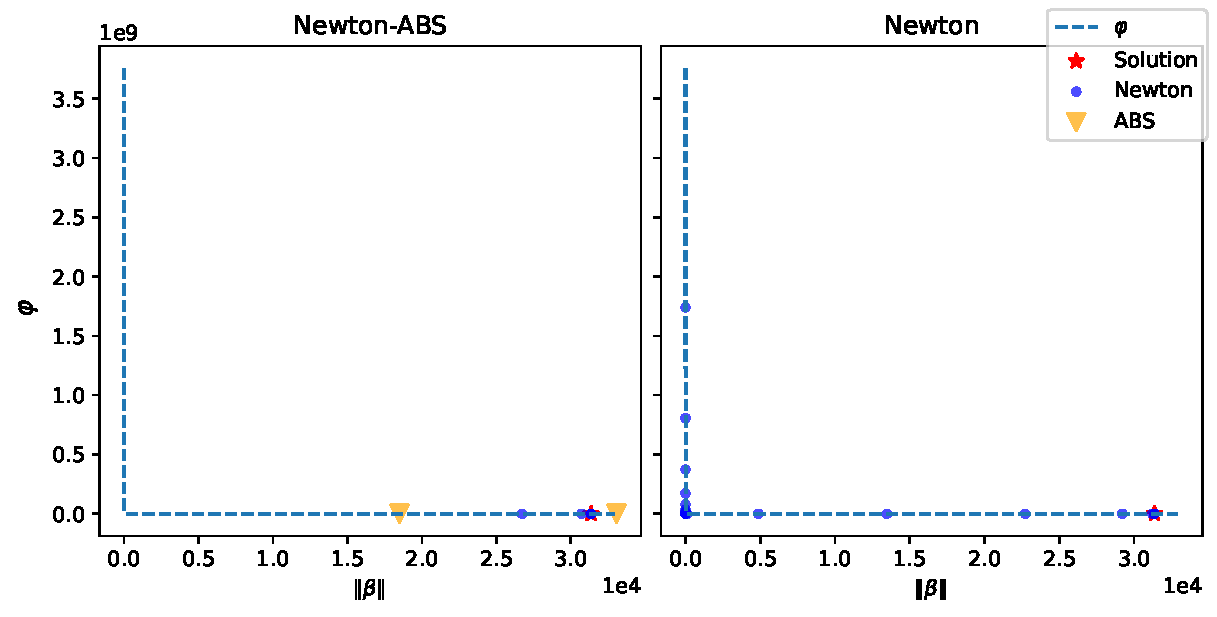
\includegraphics[width=0.7\textwidth]{figures/newton_stuck.pdf}
    \caption{Plot of Newton iterations for Newton's Method and Newton-ABS.
        It is clear from the right panel that Newton's Method struggles 
        when there is a sharp decay near the origin, since the Newton iterations
        slowly exit the kink.
        Newton-ABS goes around this problem by finding a good initial point
        sufficiently away from the origin.
    }
    \label{fig:newton-abs:stuck}
\end{figure}

\Cref{alg:nabs:nabs} is an effective way to leverage the power of both Newton Method and bisection.
Similarly, there are other methods such as Dekker's Method and Brent's Method
that combine many root-finding methods such as inverse quadratic interpolation,
secant method, and bisection method to leverage their different merits~\citep{brent:2013,dekker:1969}.
In~\Cref{fig:bench:newton-compare},
we also include benchmark results of Brent's Method
and find that Newton-ABS is superior. 
We refer to the full benchmark comparison to~\Cref{ssec:benchmark:pgd-newton}.
